\documentclass[12pt]{article}

\usepackage[letterpaper,includeheadfoot,top=1cm,bottom=2cm,left=2cm,right=2cm]{geometry}
\usepackage{here}
\usepackage{amsmath}
\usepackage{amssymb}
\usepackage{mathtools}
\usepackage{bm}
\usepackage{sectsty}
\usepackage{graphicx}
\usepackage[colorlinks=true,urlcolor=blue]{hyperref}
\usepackage{authblk}
\usepackage{caption}
\usepackage{fancyvrb}
\usepackage{relsize}
\usepackage{parskip}
\usepackage{caption}
\usepackage{subcaption}

\title{Optimizing Data Generation for Reinforcement Learning}
\author[1]{Rudra Barua}
\author[1]{Charles Harrington}
\author[1]{Fiona Henry}
\author[1]{Michael Krumdick}
\affil[1]{Harvard University}

\date{May 5, 2022}

\begin{document}

\maketitle

\begin{abstract} 
In deep reinforcement learning an agent learns a behavior by interacting with an environment. Most reinforcement learning models are built upon hyper optimized deep learning libraries, and often times the bottleneck is in generating data for model to train on rather than running the model itself. However, current practice in deep reinforcement learning does not take the efficiency of environment design in account. Through a computational study, we demonstrate how improvements in the computational efficiency of the data generation process can lead to twice as fast wall clock convergence times for applying deep reinforcement learning to chess.
\end{abstract}

\section{Background and Significance}\label{sec:background}
      
Deep Reinforcement Learning is a field of machine learning that deals with learning behaviors. In contrast to the standard supervised learning setup, these models will learn from ``experience." The models, or agents, will interact with an environment and generate data which will then be used to further optimize the model. There is no pre-existing dataset; all the data needs to be generated by the model itself. A general overview of this process is shown in Figure~\ref{fig:rl-diagram}.

\begin{figure}[H]
    \centering
    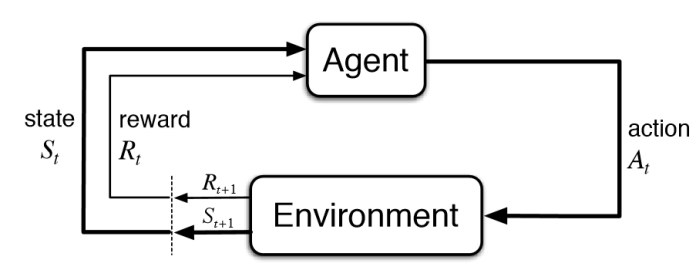
\includegraphics[width=0.5\textwidth]{plots/rl-diagram.jpg}
    \caption{Diagram of training a Reinforcement Learning model \cite{bhatt_5_2018}.}
    \label{fig:rl-diagram}
\end{figure}

These algorithms are famously sample inefficient. Even learning simple tasks can require tens of millions of samples from an environment. Most works looking at improving the efficiency of these algorithms focuses on improving the sample complexity of the model. However, the bottleneck is oftentimes in interacting with the environment.

The environment is whatever game or simulation that agent is trying to learn how to interact with. Typically, the models will be implemented using some hyper-optimized CUDA code that makes them very efficient at processing data in batches. On the other hand, the environments are oftentimes simply implemented in Python. This sequential program receives the action from the agent, steps the environment forward a single time-step, and then returns some data. In order to quickly generate data for our model, a common approach is to run these environments in in parallel. This will normally be orchestrated via Python's \texttt{multiprocessing}\footnote{\url{https://github.com/Python/cPython/tree/main/Lib/multiprocessing}} or \texttt{joblib}\footnote{\url{https://github.com/joblib/joblib}} libraries.

The paper ``Sample Factory: Egocentric 3D Control from Pixels at 100000 FPS with Asynchronous Reinforcement Learning'' was one of the main inspirations for this work. This paper analyzes potential increases in efficiency by mainly focusing on the throughput from the environment \cite{petrenko_sample_2020}. Instead of taking the normal approach and scaling the total amount of compute across many different machines, they are able to make improvements in the wall clock times of these algorithms by maximizing the efficiency on a single machine.

\section{Scientific Goals and Objectives}\label{sec:goals-and-objectives}
   
We are specifically interested in evaluating our ability to speed up the learning process for a deep reinforcement learning algorithm applied to chess. Computer scientists have been interested in developing chess playing programs since the dawn of computing. Progress in chess has largely mirrored progress in Artificial Intelligence as a whole. For the first few decades, research was focused on more traditional search and evaluation based techniques. More recently, deep learning based reinforcement learning agents have become to represent the cutting edge of these chess programs. In 2017, Deepmind's AlphaZero \cite{alphazero} deep reinforcement agent defeated the previous top chess engine, Stockfish \cite{silver_mastering_2017}. This algorithm was incredibly computationally demanding, utilizing thousands of TPU's.

In this project, we began by implementing and paralyzing chess environment generation in C++. After conducting analysis on this preliminary work (see Section~\ref{subsec:preliminary-results}), we were both excited by the results and curious about further optimizations that we could make. This led to the decision to expand our scope outside of just the environment generation to the full training process. We created a chess environment package, \texttt{chessenv}, that can be hooked up to and train a real reinforcement learning model. Results from the full system study (see Section~\ref{subsec:full-system-results}) show that using \texttt{chessenv} yields a training speed up of nearly $2\times$ compared to other top open source chess environments.

\section{Algorithms and Code Parallelization}\label{sec:algorithms-and-parallelization}

It is very typical for machine learning researchers to generate environments using multiprocessing in Python. Native Python is inherently slower than C++, however, and its multiprocessing is not as robust as OpenMP. To better understand these potential performance gaps, we created and tested sequential and parallelized implementations in both languages.

The general flow of model training is as follows. Our reinforcement learning agent interacts with the environment to generate a batch of data. The model then uses this data to perform some optimization step to increase it's performance. This process will repeat until the agent has reached an acceptable level of performance. For our initial analysis, we were interested in a batch size of 512. This means that at each step, our model must generate 512 environment interactions before it can perform an update. This can either come in the form of 512 parallel environments executing a single step, 128 parallel environments performing 4 steps, or a single sequential environment executing 512 steps. This data generation process is done using different libraries and parallelization approaches depending on which language we use. 
  
\subsection{Python Environment Generation}\label{subsec:Python-environment} 

In Python, we use the \texttt{chess}\footnote{\url{https://github.com/niklasf/Python-chess}} library as a baseline for our environment generation. This library implements the underlying chess engine that we use in order to step forward our games. We implemented two different environments using this library: a parallel and sequential version. The sequential version simply steps each environment forward one by one. The parallel version spawns a new process for each environment using Python's builtin multiprocessing module, and runs each step in parallel. The interprocess communication is implemented using a queue-based messaging mechanism. This version of the environment represents the standard practice for reinforcement learning practitioners: wrapping sequential Python code with some Python multiprocessing based library. This is due both to the dominance of Python in the machine learning space and Python's poor multi-threading performance due to the global interpreter lock (GIL).


\subsection{C++ Environment Generation}\label{subsec:cpp-environment}

In C++, we use the \texttt{libchess}\footnote{\url{https://github.com/kz04px/libchess}} library for environment generation. For each environment the chess library returns the state of chess board after the move the agent chose is applied. Again, this can occur sequentially or in parallel. Instead of relying on multi-processing to perform our parallelized step, we used a shared memory architecture and threads to minimize the overhead. 

We experimented with both shared memory parallelism using OpenMP, and distributed memory parallelism using MPI. However, due to the number of cores available on a single node and the relatively small size of our intial batch, we opted to first focus on the shared memory implementation. We designed our underlying data structure of an ``structure of arrays'' approach where we had a single environment object that contained an array of each of the current states for each environment. 

When using OpenMP, we distributed the steps among the total number of threads using a \texttt{pragma omp parallel for} statement. Notably, we are not constraining the environment to a one-thread-one-environment alignment, meaning that we could be executing the step for 128 environments with only 32 threads. In practice, we found that adding the total number of threads to match the total number of environments was often not worth the additional computational cost.

\subsection{\texttt{chessenv} Environment Generation}\label{subsec:chessenv}

We utilized a very similar design to our C++ implementation for our C-based Python module. We opted to use \texttt{MisterQueen}\footnote{\url{https://github.com/fogleman/MisterQueen}} as our underlying chess library, since it implements very efficient ``bitboard'' operations for move application and generation. We re-used the same ``structure of arrays'' shared memory architecture that we had developed for the C++ version, but adapted and optimized it for our C code.

Since we wanted to use this code to train an actual model, there were a few futher modifications that we need to make. The main one was the addition of move masking. Most reinforcement learning agents are not constrained to follow the rules of chess. This leads to a very significant frequency of illegal moves early in training. To mitigate this, most models will simply manually mask out the probabilities for invalid actions. To do so, the model needs to not only return the board at the end of every step, but also enumerate all of the possible actions, convert those actions to a unique id, and return a vector such that the valid action indices are all one while the invalid actions are all zero. Having a library with fast move generation is vital to this operation.

We also needed to make sure that we minimized the overhead for sending our data from the raw C data types into PyTorch tensors. To do so, we defined a series of operations that would convert all of our data structures into integer based representations. To send data back and forth, we would use NumPy arrays casted as pointers to integer arrays to allow our C code to directly write to the memory. Then, these NumPy arrays were directly converted into PyTorch with very little overhead.

\subsection{Specific Memory and I/O Requirements}

Our code heavily relies both on OpenMP and CUDA. The GPU memory requirements are dependent on the model size, and thus can vary with the experiment. For the environment generation, the memory requirements are very little. This is because our implementation uses only 512 environments consisting of integer vectors of length 64. There are no I/O requirements, as we are not reading anything from disk nor writing anything to disk.

\subsection{Validation, Verification} 

\subsubsection{Regression Testing}
For our Python module, we implemented a series of regression tests to verify that our underlying 
logic matched that of the well tested Python implementations. To do so, we had to implement additional transformations to convert our integer based board and move representations into their Python based analogues. However, this allow us to directly compare and verify that we were implementing the same underlying logic. 

\subsubsection{OpenSpiel Verification}\label{subsec:openspiel-verification}

\begin{figure}[H]
    \centering
    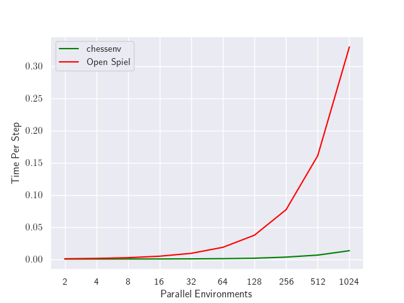
\includegraphics[width=0.6\textwidth]{plots/time_per_step.png}
    \caption{Time per step for \texttt{chessenv} vs. OpenSpiel.}
    \label{fig:time_per_step}
\end{figure}

We also benchmarked the performance of environment against the chess environment against OpenSpiel \cite{OpenSpiel}, a open source implementation of many different reinforcement leanring environments released by DeepMind. This environment represents the state of the art in terms of publicly available implementations of reinforcement learning environments for chess. Although the underlying chess engine they used for this library is also written in C++, OpenSpiel does not provide a low level mechanism for performing parallelized steps. We implemented a similar multiprocessing version to our initial parallelized Python version, but we found that this did not lead to speed ups when the number of environments was small, and quickly ran into system limits on files and processes when the number of environments was too large. 

The average speed per step of our \texttt{chessenv} environment and the OpenSpiel environment can be see in Figure~\ref{fig:time_per_step}. As you can see from this figure, our environment ended up being significantly faster. Further results and discussion can be found in Section~\ref{subsec:chessenv-performance}.


\section{Performance Benchmarks and Scaling Analysis}\label{sec:benchmarks-and-analysis}

\subsection{Preliminary Results}\label{subsec:preliminary-results}

We began our primary analysis by creating roofline models for both Intel Broadwell and Opteron AMD processors and calculating where our implementations lay on their graphs.

\begin{figure}[H]
    \centering
    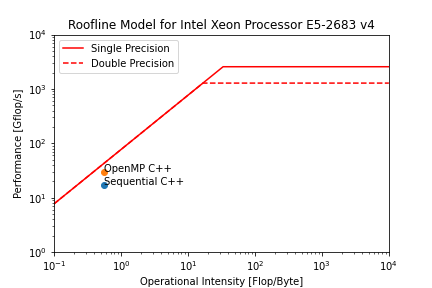
\includegraphics[width=0.6\textwidth]{plots/roofline_broadwell.png}
    \caption{Roofline analysis for Intel Xeon Processor E5-2683 v4.}
    \label{fig:roofline_broadwell}
\end{figure}

The roofline model shown in Figure~\ref{fig:roofline_broadwell} is for the Intel Xeon Processor E5-2683 v4. The base frequency of this chip is 2.1GHz, however it supports a boosted $f = 2.5$GHz for AVX2 workload. Since this chip supports AVX2, the SIMD vector width is $w_s = 256$ bits and has 4 SIMD lanes with double precision. FMA3 instructions are supported, meaning that the total flop per cycle is $\phi = 4$ Flop/cycle. Nominal peak arithmetic performance is given by
\begin{equation}
    \pi = f \times n_c \times \frac{w_s}{\mbox{precision}} \times \phi. \label{eq:peak-arithmetic}
\end{equation}
Therefore, with $n_c=32$ cores, the peak performance is
\begin{equation}
    \pi = 2.5 \times 10^9 \mbox{ cycle/s} \times 32 \times \frac{256 \mbox{ bits}}{32 \mbox{ bits}} \times 4 \mbox{ flops/cycle}  = 2560 \mbox{ Gflops/s }
\end{equation}
for single precision and
\begin{equation}
    \pi = 2.5 \times 10^9 \mbox{ cycle/s} \times 32 \times \frac{256 \mbox{ bits}}{64 \mbox{ bits}} \times 4 \mbox{ flops/cycle}  = 1280 \mbox{ Gflops/s}
\end{equation}
for double precision. Given that 64 bits move through one channel per cycle with a maximum of $c=4$ memory channels and DDR4 2400 MHz memory that operates at a frequency of $f_{DDR} = 1200$ MHz, the peak memory bandwidth is
\begin{equation}
    \beta = 2 \times f_{DDR} \times c \times w = \frac{1}{8}(2400 \times 4 \times 64) = 76.8 \mbox{ GB/s}.
\end{equation}

To determine where our sequential and parallel C++ implementations fit on this roofline, we logged the results of the Performance Application Programming Interface (PAPI) counter, shown in Table~\ref{tab:papi-results}. We compared the performance between the Sequential C++ and OpenMP C++ implementation at $N = 1,000,000$ boards. Since we assume the total instructions to all be floating point, we found the operational intensity (OI) by calculating the proportion of instructions that were floating point operations, given by the difference between the total floating point instructions and total load/store operations. Both implementations gave a similar operational intensity of $0.55$. However, we noticed the great improvement in the nominal arithmetic performance. The OpenMP implementation saw a near doubling in performance from the sequential implementation going from about $16.9$ Glop/s to about $29.8$ Glop/s. This apparent in our roofline model as the point for OpenMP C++ is shifted above the point for Sequential C++ but is around the same OI. 

\begin{table}[H]
    \centering
    \begin{tabular}{rl}
        \hline\hline
        \multicolumn{2}{c}{Hardware Counter with PAPI (1,000,000 Boards)} \\
        \hline \hline
        Total instructions & 168,871,250,061 \\
        Instructions per cycle & 1.59331 \\
        Total L1 data misses & 14,006,475  \\
        Total load/store & 108,552,964,772  \\
        OI (Flops/Byte) & 0.555657  \\
        Sequential C++ Performance [Gflop/s] & 16.91084 \\
        OpenMP C++ Performance [Gflop/s] & 29.7934 \\
        \hline \hline
    \end{tabular}
    \caption{Results of Performance Application Programming Interface (PAPI).}
    \label{tab:papi-results}
\end{table}

\begin{figure}[H]
    \centering
    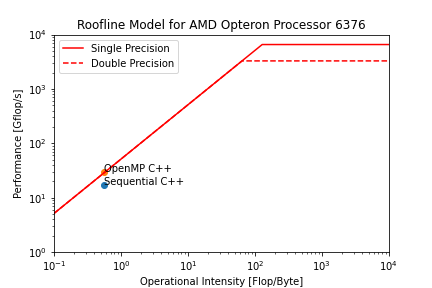
\includegraphics[width=0.6\textwidth]{plots/roofline_amd.png}
    \caption{Roofline analysis for AMD Opteron Processor 6376.}
    \label{fig:roofline-amd}
\end{figure}

The roofline model presented in Figure~\ref{fig:roofline-amd} is for the AMD Opteron Processor 6376. The base frequency of this chip is 2.3GHz, however it supports a boosted $f = 3.2$GHz for AVX2 workload. Since this chip supports AVX2, the SIMD vector width is $w_s = 256$ bits and has 4 SIMD lanes with double precision. Again, fuse multiply-add is supported, meaning the total flops per cycle is $\phi = 4$ Flop/cycle. Therefore, with $n_c=64$ cores, we can use Eq.~(\ref{eq:peak-arithmetic}) to calculate a peak arithmetic performance of
\begin{equation}
    \pi = 3.2 \times 10^9 \mbox{ cycle/s} \times 64 \times \frac{256 \mbox{ bits}}{32 \mbox{ bits}} \times 4 \mbox{ flops/cycle}  = 6553.6 \mbox{ Gflops/s}
\end{equation}
for single precision and
\begin{equation}
    pi = 3.2 \times 10^9 \mbox{ cycle/s} \times 64 \times \frac{256 \mbox{ bits}}{64 \mbox{ bits}} \times 4 \mbox{ flops/cycle}  = 3276.8 \mbox{ Gflops/s}
\end{equation}
for double precision. Given that 64 bits move through one channel per cycle with a maximum of $c=4$ memory channels and DDR3 1600 MHz memory that operates at a frequency of $f_{DDR} = 800$ MHz, the peak memory bandwidth is
\begin{equation}
    \beta = 2 \times f_{DDR} \times c \times w = \frac{1}{8}(1600 \times 4 \times 64) =  51.2 \mbox{ GB/s}.
\end{equation}
An important point about the results shown in Figure~\ref{fig:roofline-amd} is that our OpenMP implementation is right at the roofline, meaning that we memory bound. To get a better sense for this and how it could impact our ability to increase performance through parallelization, we moved on to a scaling analysis.

\begin{figure}[H]
    \centering
    \begin{subfigure}[c]{0.55\textwidth}
        \centering
        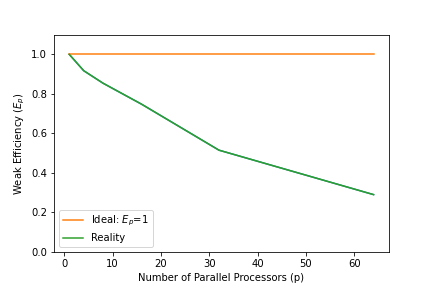
\includegraphics[width=\textwidth]{plots/weak_scaling.png}
    \end{subfigure}
    \hfill
    \begin{subfigure}[c]{0.44\textwidth}
        \centering
        \begin{tabular}{||cccc||} 
            \hline
            Threads & Boards & Time (s) & $E_p$\\ %[0.5ex] 
            \hline\hline
            1 & 100 & 0.506118 & 1.00 \\ 
            \hline
            2 & 200 & 0.520504 & 0.97 \\
            \hline
            4 & 400 & 0.551855 & 0.92\\
            \hline
            8 & 800 & 0.592725 & 0.85\\
            \hline
            16 & 1600 & 0.677184 & 0.75 \\
            \hline
            32 & 3200 & 0.982616 & 0.52\\
            \hline
            64 & 6400 & 1.74362 & 0.29\\ %[1ex] 
            \hline
        \end{tabular}
    \end{subfigure}
    \caption{Results of weak scaling analysis.}
\end{figure}

\begin{figure}[H]
    \centering
    \begin{subfigure}[c]{0.55\textwidth}
        \centering
        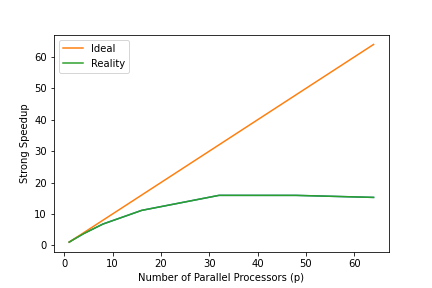
\includegraphics[width=\textwidth]{plots/strong_scaling.png}
    \end{subfigure}
    \hfill
    \begin{subfigure}[c]{0.44\textwidth}
        \centering
        \begin{tabular}{||cccc||} 
            \hline
            Threads & Boards & Time (s) & $S_p$\\ %[0.5ex]
            \hline\hline
            1 & 512 & 2.56208 & 1.00\\
            \hline
            2 & 512 & 1.32137 & 1.94\\
            \hline
            4 & 512 & 0.689421 &  3.72\\
            \hline
            8 & 512 & 0.378254 &  6.77\\
            \hline
            16 & 512 & 0.230451 & 11.12\\
            \hline
            32 & 512 & 0.161108 & 15.90\\
            \hline
            48 & 512 & 0.161188 & 15.89\\
            \hline
            64 & 512 & 0.168011 & 15.24\\ % [1ex]
            \hline
        \end{tabular}
    \end{subfigure}
    \caption{Strong Scaling Analysis}
\end{figure}

The results of our scaling analysis show us that after about 32 cores, we do not achieve much more speed up. This matches what we expected given the results of our roofline analysis. Thus, it does not make sense to use more than 32 to cores to generate our environments. In order to gain more performance within the environments, we need to move right on the roofline plots by increasing our memory performance. Doing this would require us to abandon the \texttt{chesslib} library and develop our own base implementation, however. Before doing this, we determined that it was important to expand our scope to the entire system and evaluate performance improvement.

\subsection{Full System Results}\label{subsec:full-system-results}

In order to evaluate the performance of our implementations in the context of the entire system, we generated the plot shown in Figure~\ref{fig:batch_throughput}. Note that this plot includes our Python implementations as outlined in Section~\ref{subsec:Python-environment}.

\begin{figure}[H]
    \centering
    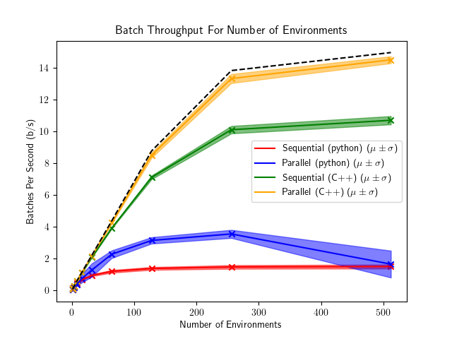
\includegraphics[width=0.6\textwidth]{plots/batch_throughput.png}
    \caption{Batch throughput of different implementations. The dashed black line represents the batch throughput for an ideal environment with instantaneous data generation.}
    \label{fig:batch_throughput}
\end{figure}

The previous weak and strong scaling analyses were conducted only on the data generation part of the system. Recall that there is a back-and-forth nature between the environment and the agent. The environment generates a batch of data and passes it to the agent, who then executes inference and updates and passes moves back to the environments for more data generation, and so on. Figure~\ref{fig:batch_throughput} shows the results from the full system scaling analysis. This graphic shows the throughput of the entire system, measured by the number of batches processes per second as we increase the number of environments used. The dashed black line represents the theoretical maximum, which would occur when the data generation is executed instantaneously. As we'd expect, both Python implementations are outperformed by even sequential C++. Our shared-memory parallelism achieves near-ideal performance, indicated by its close proximity to the theoretical maximum. This tells us that our bottleneck has shifted from the environment generation to the model inference. To address this, we looked for ways to optimize the model, beginning with choosing a smaller model that takes in a larger batch size. Details of our resulting \texttt{chessenv} package are discussed in Section~\ref{subsec:chessenv}.

\subsection{\texttt{chessenv} Performance Benchmarking}\label{subsec:chessenv-performance}

To benchmark the performance of \texttt{chessenv} library, we compared it to that of OpenSpiel. Figure~\ref{fig:time_per_step} shows an initial comparison of the two used for verification of our implementation. To compare overall system performance, we generated the plots seen in Figures~\ref{subfig:time-per-update} and~\ref{subfig:efficiency}.

\begin{figure}[H]
    \centering
    \begin{subfigure}[c]{0.49\textwidth}
        \centering
        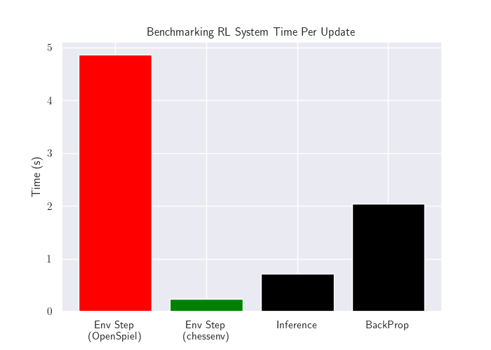
\includegraphics[width=\textwidth]{plots/benchmark.png}
        \caption{Time per update}
        \label{subfig:time-per-update}
    \end{subfigure}
    \begin{subfigure}[c]{0.49\textwidth}
        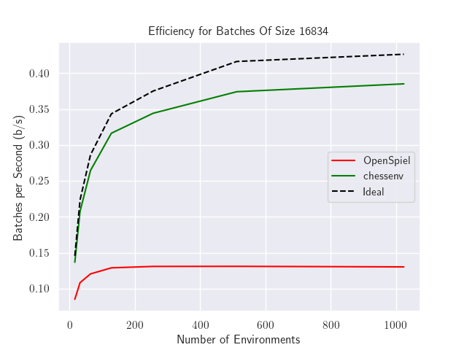
\includegraphics[width=\textwidth]{plots/efficiency.png}
        \caption{Throughput}
        \label{subfig:efficiency}
    \end{subfigure}
    \caption{Comparing performance and efficiency of \texttt{chessenv} and OpenSpiel.}
    \label{fig:openspiel-comparison}
\end{figure}

Figure~\ref{subfig:time-per-update} compares the time per update for both systems. The two black bars represent the areas of the model that are not immediately available for performance improvement, namely the inference and back propagation steps. The red and green bars show the time per environment step for OpenSpiel and \texttt{chessenv} respectively. We can see that our implementation greatly outperforms OpenSpiel. Figure~\ref{subfig:efficiency} likewise demonstrates that \texttt{chessenv} is the superior library. This plot shows the same metric as Figure~\ref{fig:batch_throughput} as well as the fact that our implementation nears the theoretical maximum again.

\begin{figure}[H]
    \centering
    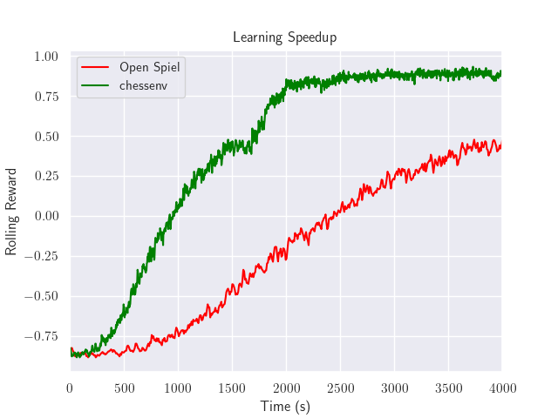
\includegraphics[width=0.6\textwidth]{plots/learning_speedup.png}
    \caption{Learning speedup of \texttt{chessenv} vs. OpenSpiel.}
    \label{fig:learning_speedup}
\end{figure}

Our final benchmark comparison is that of the learning speedup between the two libraries, shown in Figure~\ref{fig:learning_speedup}. This once again shows that \texttt{chessenv} dramatically outperforms OpenSpiel; the former achieving a rolling reward of zero in less than 1,000 seconds while the latter does the same in almost 2,500 seconds. In other words, our implementation is nearly two and a half times as efficient.

Our benchmark figures for the whole system were created using an NVIDIA Ampere A100 GPU to do Reinforcement Learning inference and 1 compute node with 4 threads for environment generation. Further information on these workflow parameters is summarized in Table~\ref{table:workflow_parameters}. 

\begin{table}[H]
    \centering
    \begin{tabular}{rr}
        \hline\hline
        Typical wall clock time (hours) & 2 \\
        Typical job size (compute node)  & 1  \\
        Typical job size (GPU) & 1  \\
        Memory per node (GB) & 40  \\
        Maximum number of input files in a job & 2 \\
        Maximum number of output files in a job & 1  \\
        \hline\hline
    \end{tabular}
    \caption{Workflow parameters for RL training during development.}
    \label{table:workflow_parameters}
\end{table}

\section{Resource Justification}\label{sec:resource-justification}

Our deep reinforcement learning example demonstrated training an agent against a simple random opponent. In order to truly verify the value of our approach, we need to benchmark against a serious deep reinforcement learning system. To do so, we propose recreating the results from the AlphaZero paper using our environment as the data generation mechanism. Although their code has never been released, it is fair to assume that it mimics the implementation that we see in OpenSpiel since they were both developed by the same organization. 

In the original algorithm, training was for 700k steps of mini batches of size 4096. Their overall training time took roughly 24 hours. They used 5,000 TPU nodes for data generation and 64 TPU nodes for training. However, since we benchmarked all of our data on GPUs, we will use another open source implementation of the same algorithm called ELF OpenGo \cite{opengo}. For their implementation, they used 2000 training workers with two Intel Xeon E5-2686 v4 processors and one V100 GPU for the data generation process, and one training worker with 8 V100 GPUs for the model training process. Although it is not specified in the paper, our experiments have demonstrated that 4 CPU cores may be enough to saturate a model. We are requesting an identical amount of compute, and we will attempt to benchmark how much faster we can train a model to the same level of performance. Given the information that we have so far, we estimate that we should be able to reduce the training time by 25-50\%, just by using \texttt{chessenv}. Since we know that it will take at most 24 hours, and we have 2001 nodes, we are requesting at most 48024 node hours.

\bibliographystyle{abbrv}
\bibliography{references}

\end{document}

% vim-local: LaTeX
